\documentclass[12pt]{article}
\usepackage[paper=letterpaper,margin=1.5cm]{geometry}
\usepackage{amsmath}
\usepackage{amssymb}
\usepackage{amsfonts}
\usepackage{mathtools}
%\usepackage[utf8]{inputenc}
%\usepackage{newtxtext, newtxmath}
\usepackage{lmodern}     % set math font to Latin modern math
\usepackage[T1]{fontenc}
\renewcommand\rmdefault{ptm}
%\usepackage{enumitem}
\usepackage[shortlabels]{enumitem}
\usepackage{titling}
\usepackage{graphicx}
\usepackage[colorlinks=true]{hyperref}
\usepackage{setspace}
\usepackage{subfigure} 
\usepackage{braket}
\usepackage{color}
\usepackage{tabularx}
\usepackage[table]{xcolor}
\usepackage{listings}
\usepackage{mathrsfs}
\usepackage{stackengine}
\usepackage{physics}
\usepackage{afterpage}
\usepackage{pdfpages}
\usepackage[export]{adjustbox}
\usepackage{biblatex}

\setstackEOL{\\}

\definecolor{dkgreen}{rgb}{0,0.6,0}
\definecolor{gray}{rgb}{0.5,0.5,0.5}
\definecolor{mauve}{rgb}{0.58,0,0.82}


\lstset{frame=tb,
  language=Python,
  aboveskip=3mm,
  belowskip=3mm,
  showstringspaces=false,
  columns=flexible,
  basicstyle={\small\ttfamily},
  numbers=none,
  numberstyle=\tiny\color{gray},
  keywordstyle=\color{blue},
  commentstyle=\color{dkgreen},
  stringstyle=\color{mauve},
  breaklines=true,
  breakatwhitespace=true,
  tabsize=3
}
\setlength{\droptitle}{-6em}

\makeatletter
% we use \prefix@<level> only if it is defined
\renewcommand{\@seccntformat}[1]{%
  \ifcsname prefix@#1\endcsname
    \csname prefix@#1\endcsname
  \else
    \csname the#1\endcsname\quad
  \fi}
% define \prefix@section
\newcommand\prefix@section{}
\newcommand{\prefix@subsection}{}
\newcommand{\prefix@subsubsection}{}
\renewcommand{\thesubsection}{\arabic{subsection}}
\makeatother
\DeclareMathOperator*{\argmin}{argmin}
\newcommand{\partbreak}{\begin{center}\rule{17.5cm}{2pt}\end{center}}
\newcommand{\alignbreak}{\begin{center}\rule{15cm}{1pt}\end{center}}
\newcommand{\tightalignbreak}{\vspace{-5mm}\alignbreak\vspace{-5mm}}
\newcommand{\hop}{\vspace{1mm}}
\newcommand{\jump}{\vspace{5mm}}
\newcommand{\R}{\mathbb{R}}
\newcommand{\C}{\mathbb{C}}
\newcommand{\N}{\mathbb{N}}
\newcommand{\G}{\mathbb{G}}
\renewcommand{\S}{\mathbb{S}}
\newcommand{\bt}{\textbf}
\newcommand{\xdot}{\dot{x}}
\renewcommand{\star}{^{*}}
\newcommand{\ydot}{\dot{y}}
\newcommand{\lm}{\mathrm{\lambda}}
\renewcommand{\th}{\theta}
\newcommand{\id}{\mathbb{I}}
\newcommand{\si}{\Sigma}
\newcommand{\Si}{\si}
\newcommand{\inv}{^{-1}}
\newcommand{\T}{^\intercal}
\renewcommand{\tr}{\text{tr}}
\newcommand{\ep}{\varepsilon}
\newcommand{\ph}{\varphi}
%\renewcomand{\norm}[1]{\left\lVert#1\right\rVert}
\definecolor{cit}{rgb}{0.05,0.2,0.45}
\addtolength{\jot}{1em}
\newcommand{\solution}[1]{

\noindent{\color{cit}\textbf{Solution:} #1}}

\newcounter{tmpctr}
\newcommand\fancyRoman[1]{%
  \setcounter{tmpctr}{#1}%
  \setbox0=\hbox{\kern0.3pt\textsf{\Roman{tmpctr}}}%
  \setstackgap{S}{-.9pt}%
  \Shortstack{\rule{\dimexpr\wd0+.1ex}{.9pt}\\\copy0\\
              \rule{\dimexpr\wd0+.1ex}{.9pt}}%
}

\newcommand{\Id}{\fancyRoman{2}}

% Enter the specific assignment number and topic of that assignment below, and replace "Your Name" with your actual name.
\title{STAT 31050: Homework 4}
\author{Caleb Derrickson}
\date{May 8, 2024}

\begin{document}
\onehalfspacing
\maketitle
\allowdisplaybreaks

\tableofcontents

\newpage
\section{Exercise 22}
Consider the integral operator $T: L^2[-1, 1] \to L_2[-1, 1]$ defined by
\[T[f](x) = \int_{-1}^1 e^{-(x - y)^2} f(y) \ dy, \ x \in [-1, 1]\]
\subsection{Exercise 22, part 1}
Prove that $T[f]$ is continuous if $f \in L_2[-1, 1]$. 
\vspace{-6mm}\partbreak
\begin{solution}

    Here, I will take a page from functional analysis, showing that the operator $T$ is bounded, linear, and maps continuous functions to continuous functions. Note that it is sufficient to show $T$ being a bounded linear operator, since it is continuous by virtue of this fact. To show linearity, let $f, g \in L^2[-1, 1]$, and $\alpha, \beta \in \R$. Then, 
    \begin{align*}
        T[\alpha f+\beta g] &= \int_{-1}^1 e^{-(x - y)^2}\qty[\alpha f + \beta g](y) \ dy = \alpha\int_{-1}^1 e^{-(x - y)^2}f(y) \ dy + \beta\int_{-1}^1 e^{-(x - y)^2} g(y) \ dy\\
        &= \alpha T[f](x) + \beta T[g](x).
    \end{align*}
    Next, we show boundedness of $T$. First, since suppose $f \in L^2[-1, 1]$, its norm is well defined in the $L^2$ sense. We will show that $\norm{T[f]}_{L^2} \leq M\norm{f}_{L^2}$. Then, 
    \begin{align*}
        \norm{T[f]}_{L^2} &= \int_{-1}^1 \qty|\int_{-1}^1 e^{-(x - y)^2}f(y) \ dy |^2 \ dx\\ 
        &\leq \int_{-1}^1 \int_{-1}^1 \qty|e^{-(x - y)^2}f(y)|^2 \ dy \ dx \\
        & \leq \int_{-1}^1 \int_{-1}^1 \qty(\sup_{y \in [-1, 1]} \qty|e^{-(x - y)^2}|^2)\qty|f(y)|^2 \ dy \ dx\\
        & \leq \qty(\sup_{x, y \in [-1, 1]}\qty|e^{-(x - y)^2}|^2)\int_{-1}^1 \int_{-1}^1 \qty|f(y)|^2 \ dy \ dx\\
        &= 2\qty(\sup_{x, y \in [-1, 1]}\qty|e^{-(x - y)^2}|^2) \int_{-1}^1 \qty|f(y)|^2 \ dy\\
        &= M\norm{f}_{L^2}
    \end{align*}
    Where $M$ is the sup squared of the given exponential. Note that the sup of the exponential is easy to find : since the squared exponential cannot be larger than one, $M$ = 1. Therefore, the mapping is bounded and hence continuous. 
\end{solution}

\newpage
\subsection{Exercise 22, part 2}
Using a Gauss-Legendre quadrature rule, write a code that discretizes the integral using a 40 point Gauss-Legendre quadrature and evaluates it at arbitrary points $x \in [-1, 1]$. You may assume $f$ is continuous. Plot the output for $f \equiv 1$ and $f \equiv x$. Then, increase the number of nodes to 80 and compare the output with the 40 point rule. 
\partbreak
\begin{solution}

   I have implemented the Gauss-Legendre rule in Python, and have used it to integrate the given functions. My results are given below. Due the fast convergence of the integration, I have also provided the errors for the two below. After these plots, I will provide my code.
\end{solution}
\vspace{0.5in}
\begin{figure}[!ht]
    \centering
    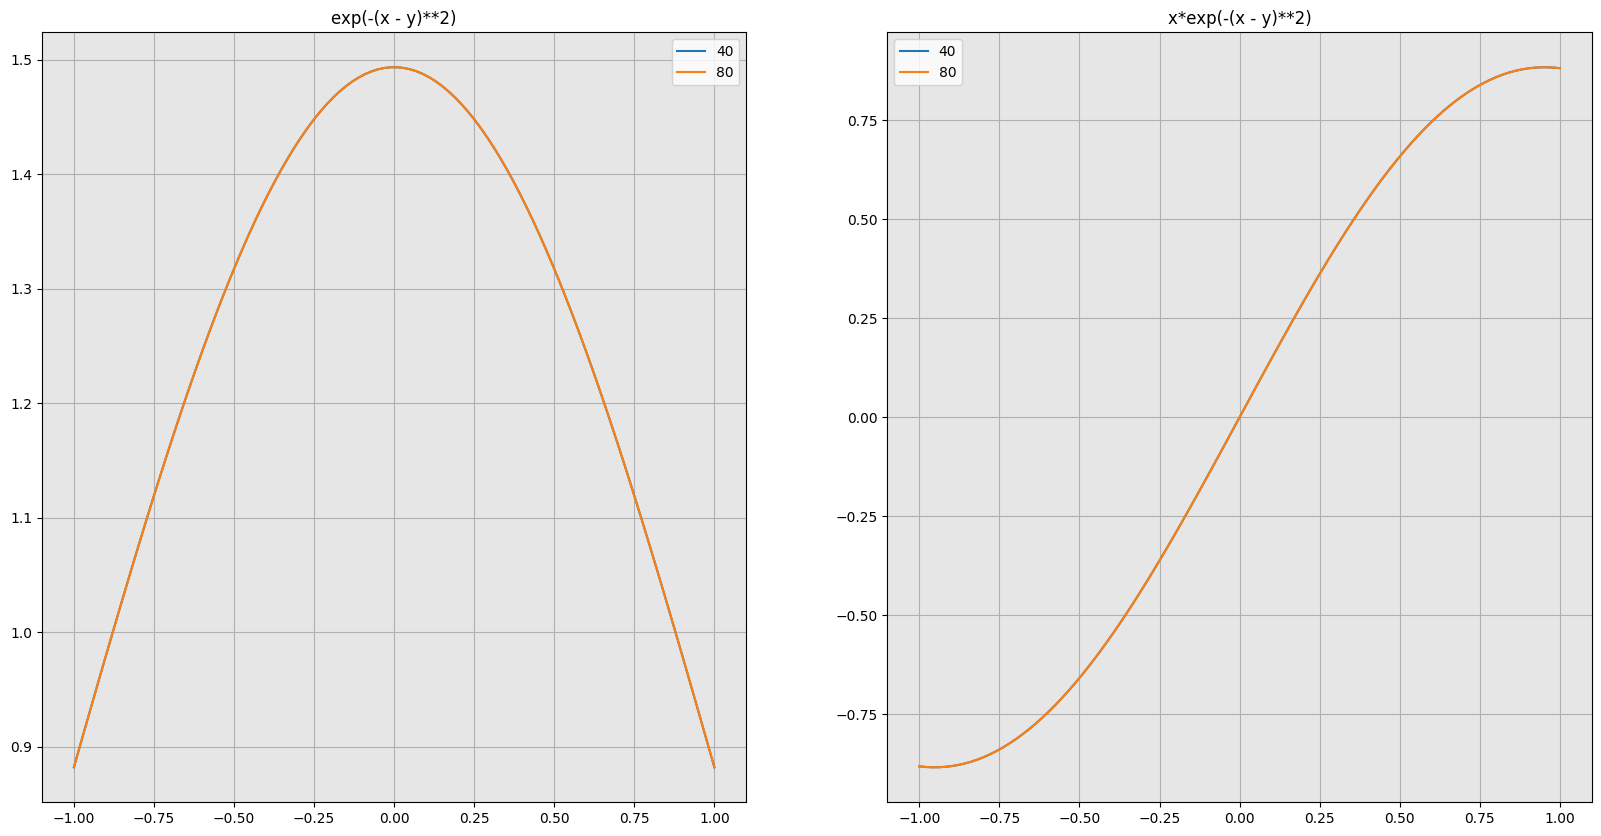
\includegraphics[width = 0.6\textwidth]{Plots/Exercise 22b1.png}
    \caption{Gauss - Quadrature with $n = 40, 80$ for the two functions.}
    \label{fig:Exercise 22b1}
\end{figure}
\begin{figure}[!ht]
    \centering
    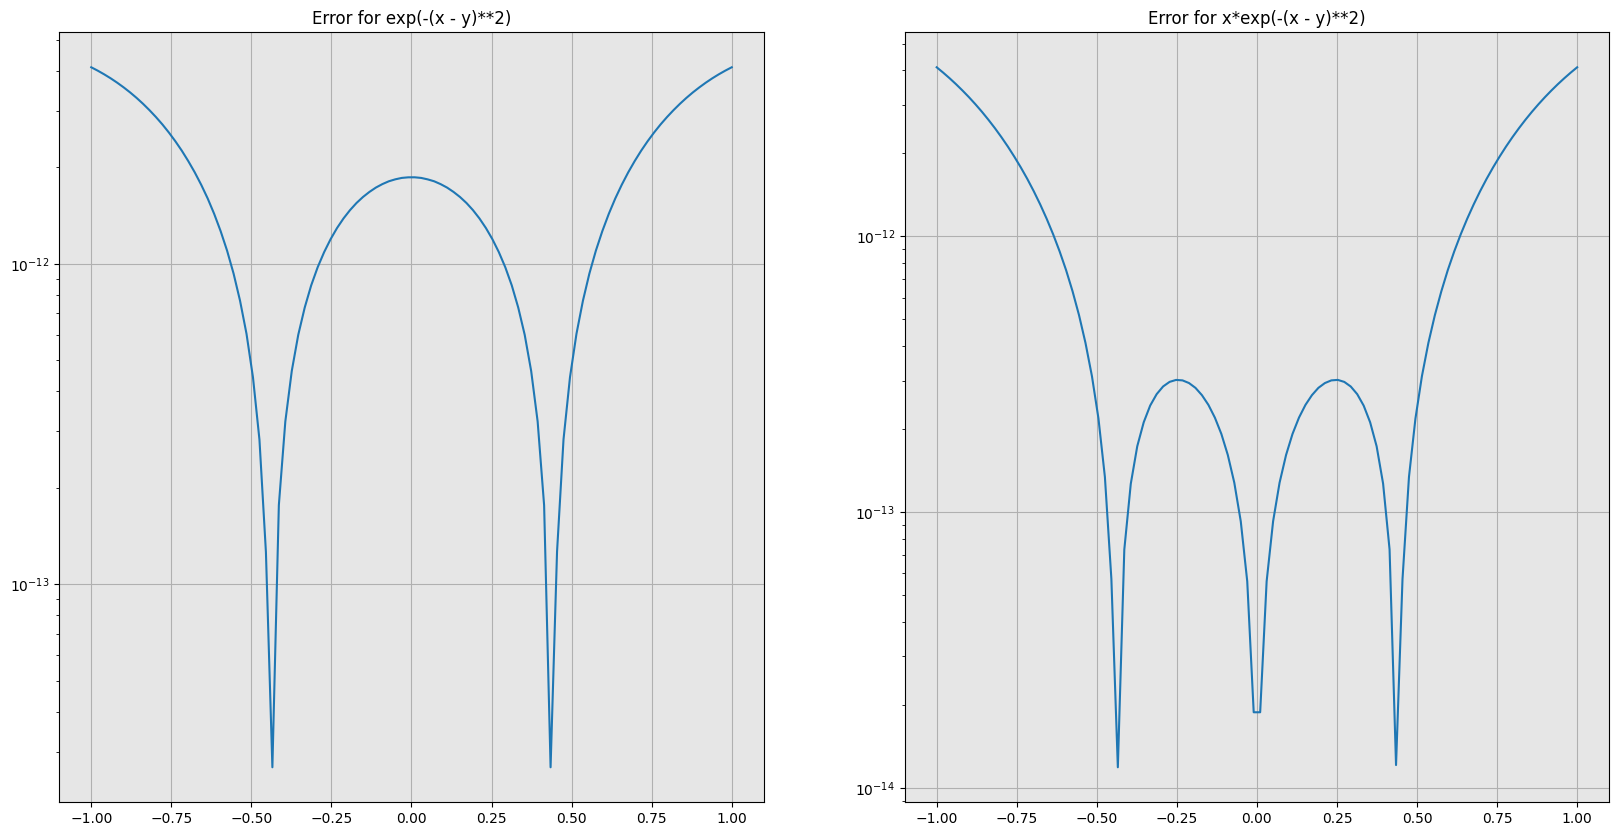
\includegraphics[width = 0.6\textwidth]{Plots/Exercise 22b2.png}
    \caption{Relative difference between the two integrations.}
    \label{fig:Exercise 22b2}
\end{figure}
\newpage
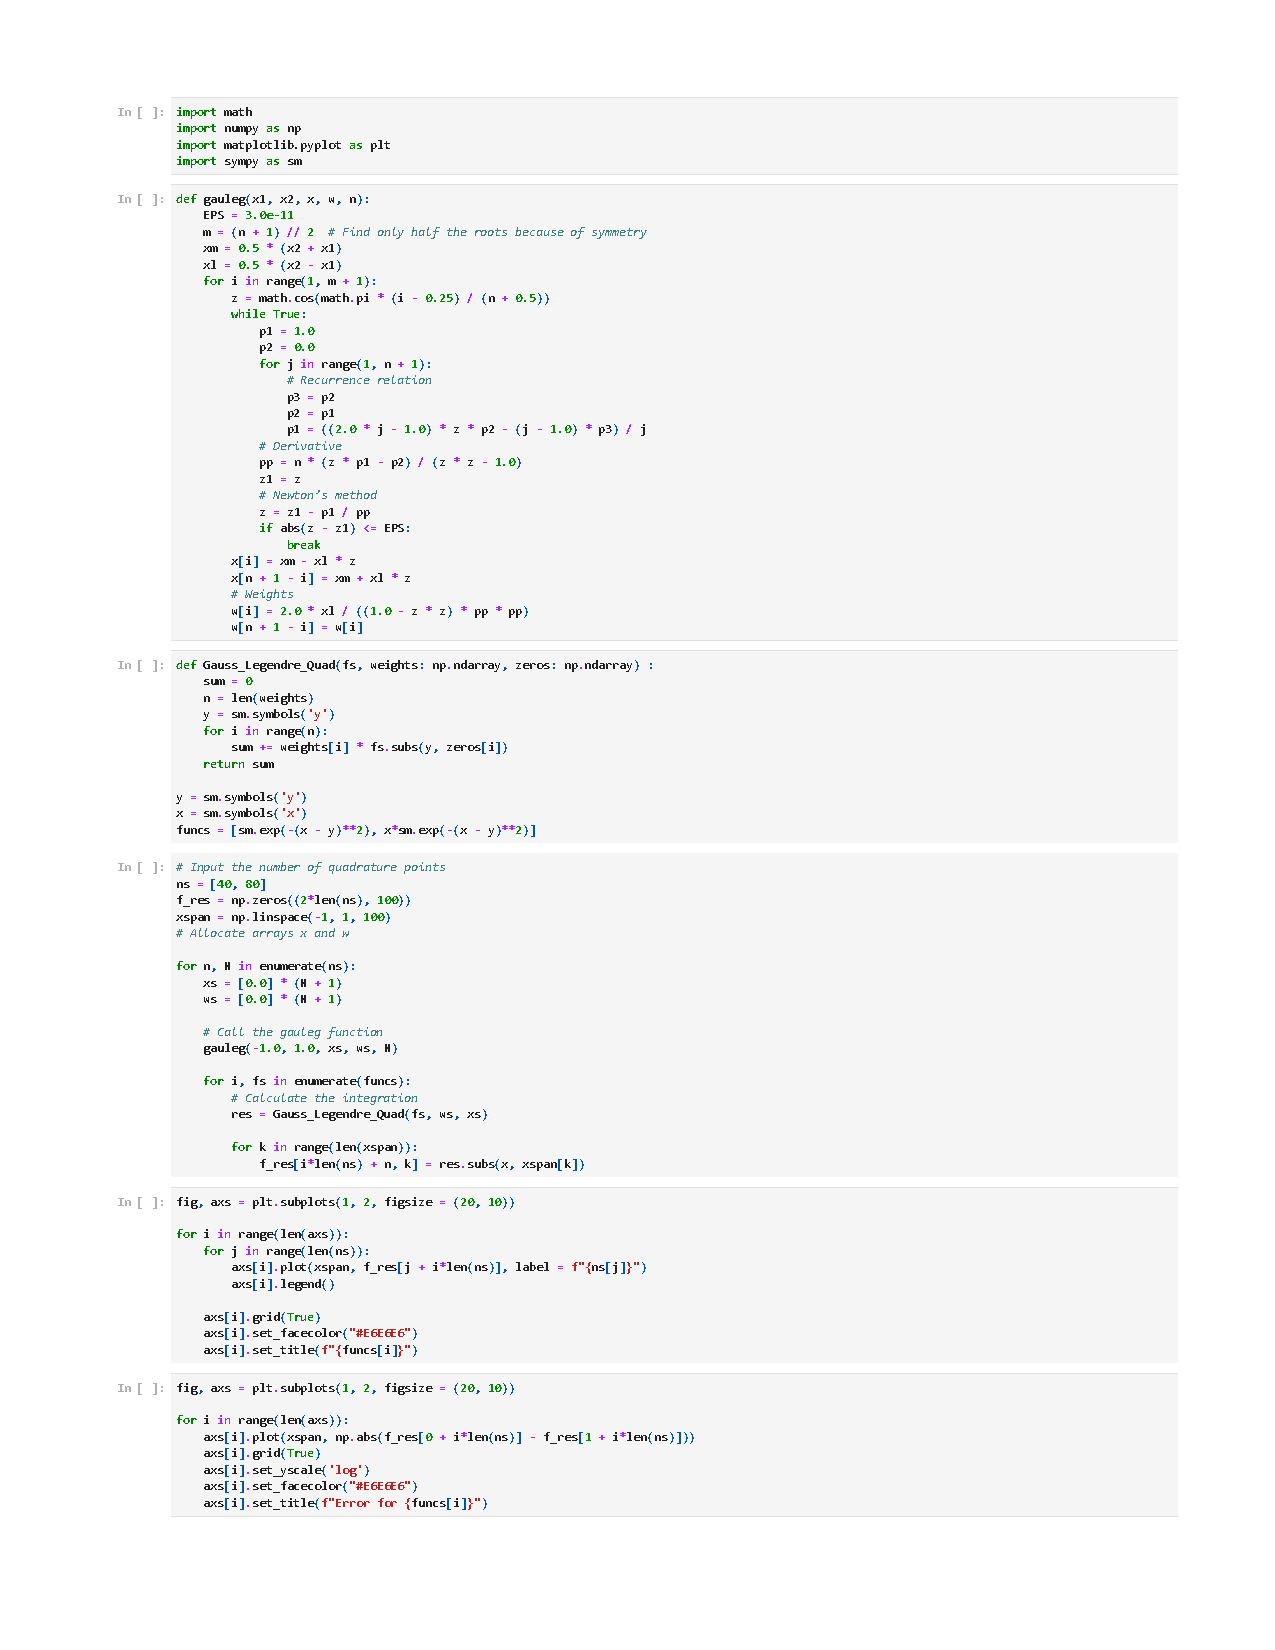
\includepdf{CodePDFs/Exercise22b.pdf}

\newpage
\subsection{Exercise 22, part 3}
Construct the matrix that takes $f$ sampled at an $n$ point Gauss-Legendre rule and maps it to $T[f]$ evaluated at the same points, i.e., $K$ maps $(f(x_1), ..., f(x_n))$ (approximately) to $(T[f](x_1), ..., T[f](x_n))$. Diagonalize $K$ with $n = 40$ and plot all eigenvalues and the first 4 eigenfunctions. Now set $n = 80$ and repeat. Compare the eigenvalues for $n = 40$ and $n = 80$. What does this say about the original integral operator $T$? You don't need to be very precise here.
\partbreak
\begin{solution}

    At any given $x$, Gauss-Legendre integration will look like (for these functions)
    \[T[f](x) =  \int_{-1}^1 e^{-(x - y)^2}f(y) \ dy \approx \sum_{i = 1}^n e^{-(x - y_i)^2}f(y_i)w_i \]
    When sampling $T[f](x)$ at the $n$ nodes obtained from the Gauss-Legendre rule, we will get 
    \[T[f](x_j) = \sum_{i = 1}^n e^{-(x_j - y_i)^2}f(y_i) w_i\]
    The matrix $K$ will then have entries $K_{i, j} = e^{-(x_j - y_i)^2}w_i$. After constructing the matrices, extracting the eigenvalues, we get the two plots below. It really seems as though there is no true difference between the two methods, since the spectrum bottoms out after $n = 15$. Also, it seems as though the two functions have the same spectrum (For the spectrum, I am taking the absolute value of the eigenvalues, since we have to worry about complex numbers). My code to generate these two plots will be given afterwards. 
\end{solution}
\vspace{0.4in}
\begin{figure}[!ht]
    \centering
    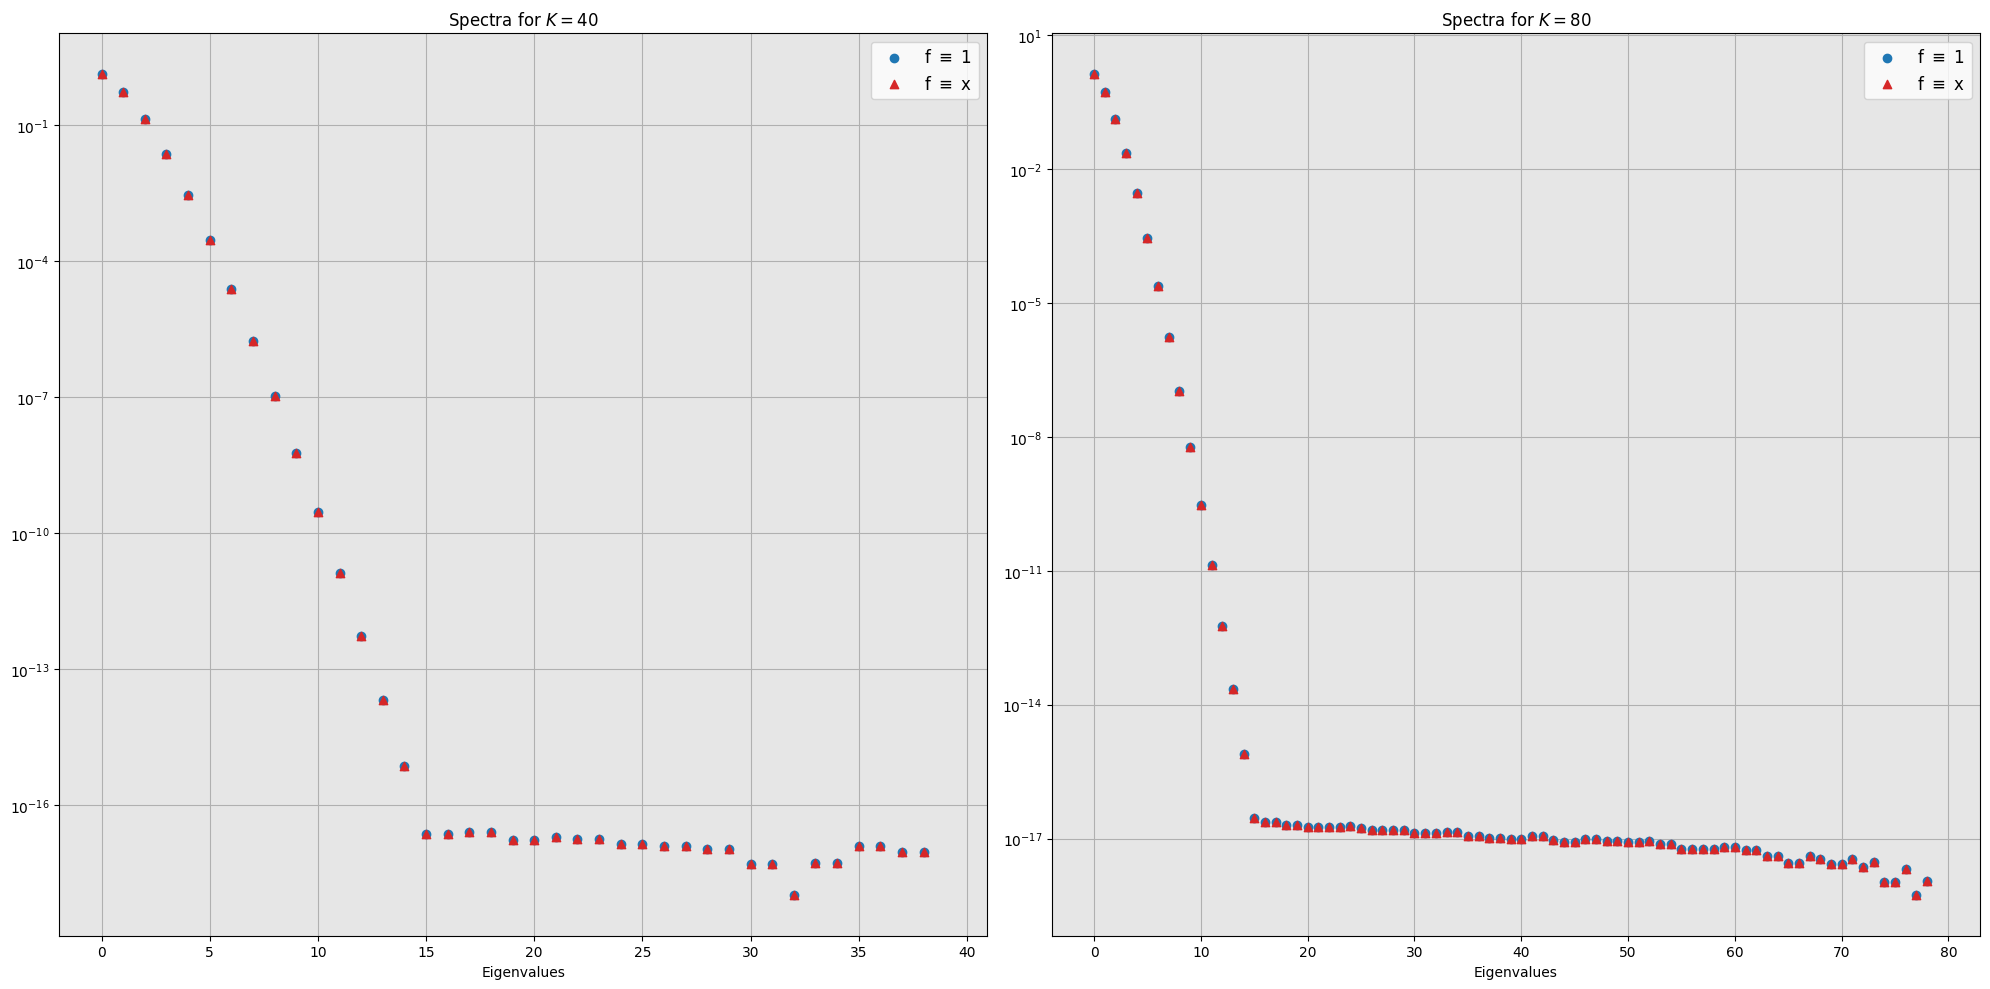
\includegraphics[width = 0.8\textwidth]{Plots/Exercise 22c.png}
    \caption{Spectrum for the Operator for $N = 40, 80$.}
    \label{fig:Exercise 22c}
\end{figure}
\newpage
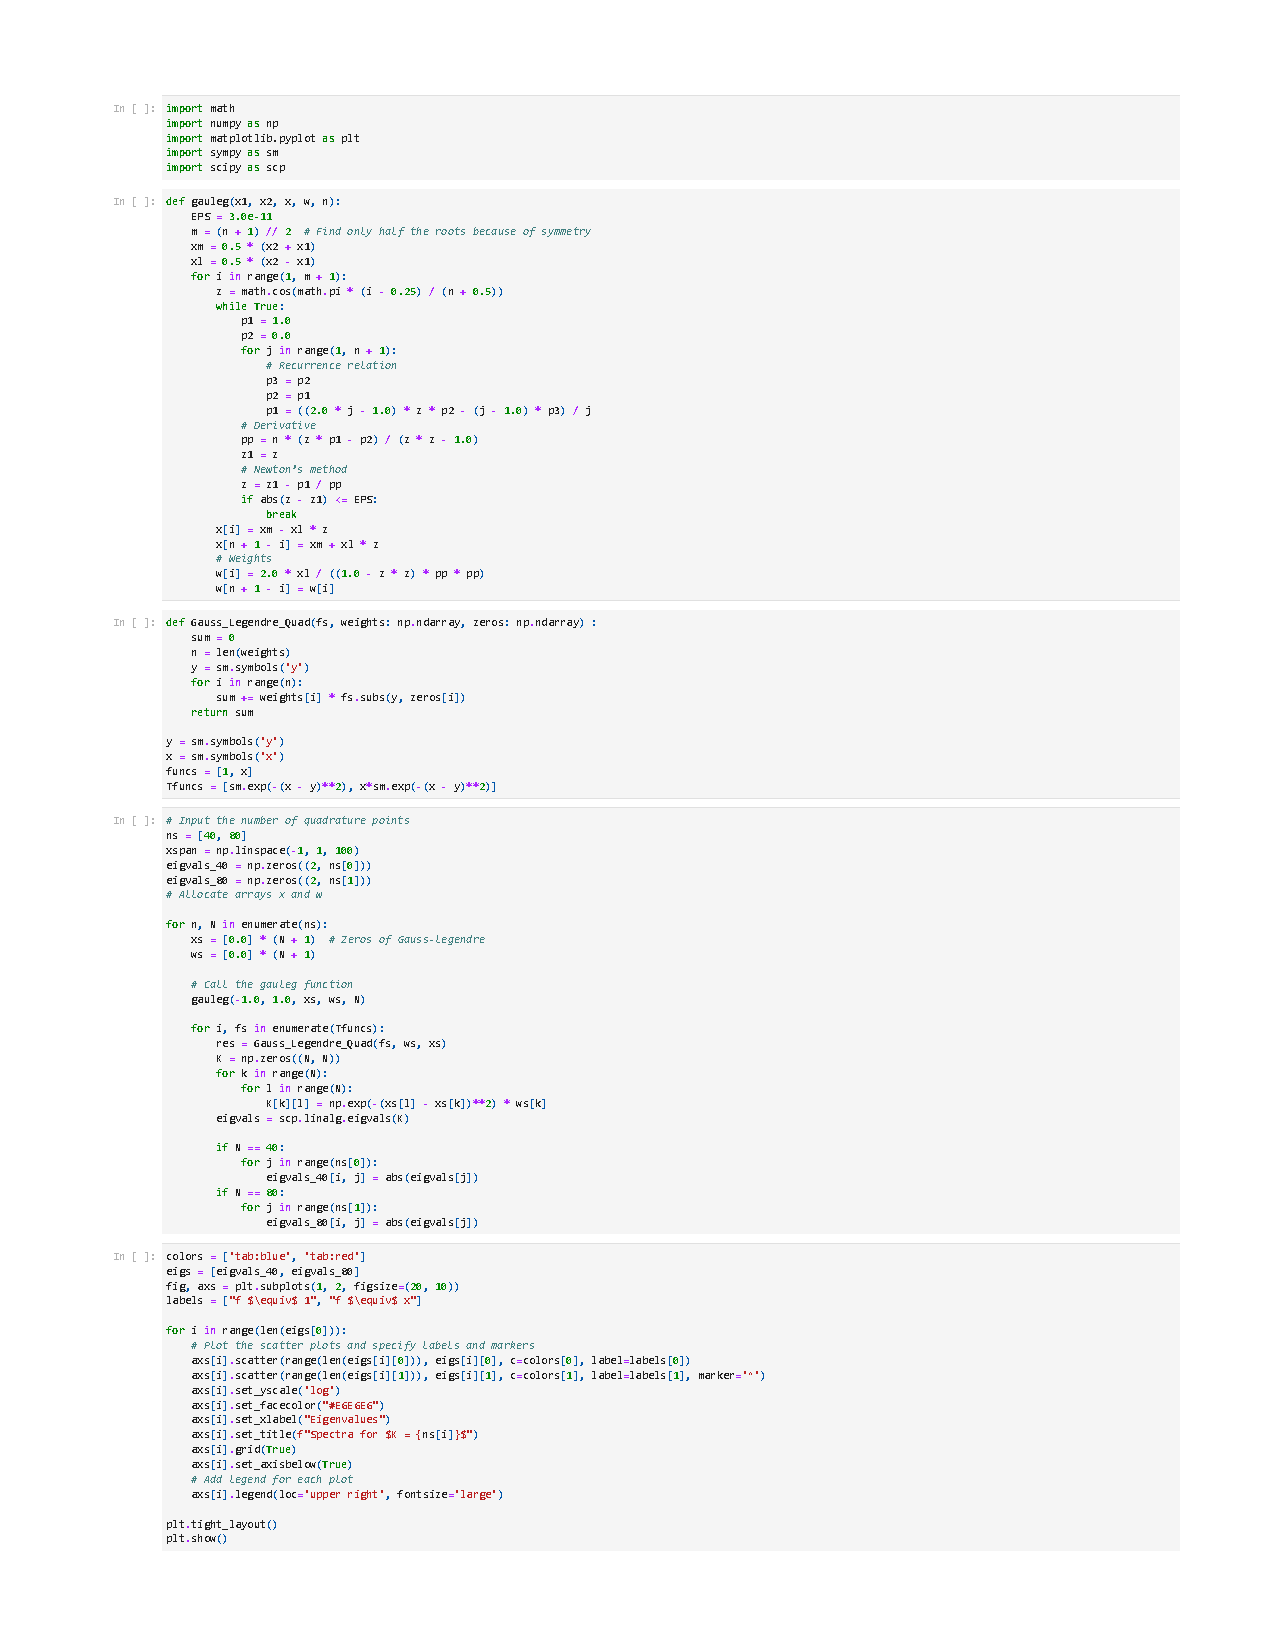
\includepdf{CodePDFs/Exercise22c.pdf}

\newpage
\section{Exercise 23}
In this problem we will play around with polynomial root finding. In the following suppose that $q_n$, $n = 0, 1, 2, ...$,  is a sequence of polynomials which satisfies a three-term recurrence 
\[q_{n+1}(x) = (\alpha_nx + \beta_n)q_n(x) + \gamma_nq_{n-1}(x), \ n > 0,\]
where $\alpha_n, \beta_n,$ and $\gamma_n$ are real numbers and the $\alpha_n$ are bounded away from zero. Also, suppose $q_1 = (a_0x + b_0)q_0(x).$ Suppose $p$ is a polynomial with 
\[p(x) = \sum_{j = 0}^n c_jq_j(x),\]
for some coefficients $c_0, ..., c_n$ with $c_n \neq 0$. Hint: if you get stuck, look at Trefethen’s book Approximation Theory and Approximation Practice, Chapter 18, but try not to!

\subsection{Exercise 23, part 1}
Find a linear map which sends the vector 
\[v = [q_0(x), q_1(x), ..., q_{n-1}(x)]^T\]
to
\[[xq_0(x), xq_1(x), ..., xq_{n-2}(x), xq_{n - 1} - q_n / \alpha_{n-1}]^T\]
for all $x \in [-1, 1]$. Your matrix should not depend on $x$. Is this map unique (assuming the independence of $x$)?
\partbreak
\begin{solution}

    Define $T$ as our linear map. Let us examine the first element. If we impose the condition above, then we have $Tq_0 = xq_0$. We also have the initial recurrence relation, given above. If we isolate the $xq_0$ term in the recurrence, we obtain
    \[Tq_0 = xq_0 = \frac{1}{\alpha_0}q_1 - \frac{\beta_0}{\alpha_0}q_0\]
    Since this equation neatly maps linear combinations of the components of $v$, we can define the first row of $T$ as such. For the general recurrence, note that we can shuffle it around via the following:
    \begin{align*}
        &q_{n+1} = \alpha_nx q_n +\beta_nq_n + \gamma_n q_{n-1}\\
        &\alpha_nxq_n= -\gamma_n q_{n-1} - \beta_n q_n + q_{n+1}\\
        &xq_n = -\frac{\gamma_n}{\alpha_n}q_{n-1} - \frac{\beta_n}{\alpha_n}q_n + \frac{1}{\alpha_n}q_{n+1}
    \end{align*}
    Then for intermediate $n$, we can write our mapping $T$ as 
    \[Tq_n = -\frac{\gamma_n}{\alpha_n}q_{n-1} - \frac{\beta_n}{\alpha_n}q_n + \frac{1}{\alpha_n}q_{n+1}\]
    This is again a linear combination of the components of $v$, so we can define the intermediate rows of $T$ as such. Note that we cannot do this for the last coordinate of $v$, since there is clearly no final $q_{n+1}$. Getting the last row, we can examine the recurrence formula for $q_n$. 
    \begin{align*}
        q_n = \alpha_{n-1}xq_{n-1} + \beta_{n-1}q_{n-1} + \gamma_{n-1}q_{n-2}\\
        q_n= \alpha_{n-1}xq_{n-1} + \beta_{n-1}q_{n-1} + \gamma_{n-1}q_{n-2}\\
         - \gamma_{n-1}q_{n-2}- \beta_nq_{n-1}= - q_n + \alpha_{n-1}xq_{n-1}\\
         - \frac{\gamma_{n-1}}{\alpha_{n-1}}q_{n-2}-\frac{\beta_{n-1}}{\alpha_{n-1}}q_{n-1} = xq_{n-1} - q_n / \alpha_{n-1}
    \end{align*}
     Therefore, solely by the recurrence formula, we have found a linear combination of the components of $v$ to form the desired output. The matrix $T$ is therefore
    \[T = \mqty[
        \frac{\beta_0}{\alpha_0}&\frac{1}{\alpha_0}&0&...&...&0\\
        \frac{-\gamma_1}{\alpha_1}&-\frac{\beta_1}{\alpha_1}& \frac{1}{\alpha_1}&0&...&0\\
        \dots\\
        0&...&0&-\frac{\gamma_{n-1}}{\alpha_{n-1}}&-\frac{\beta_{n-1}}{\alpha_{n-1}}&\frac{1}{\alpha_{n-1}}\\
        0&...&0&0&-\frac{\gamma_{n-1}}{\alpha_{n-1}}&-\frac{\beta_{n-1}}{\alpha_{n-1}}
        ].\]
\end{solution}

\newpage
\subsection{Exercise 23, part 2}
Show that $x\star$ is a root of $p$ if and only if $q_n(x\star) = -\frac{1}{c_n}\sum_{j = 0}^{n-1}c_jq_j(x\star).$
\partbreak
\begin{solution}

    I will start with the backward implication, as that is almost immediate.
    \[q_n(x\star) = -\frac{1}{c_n}\sum_{j = 0}^{n-1}c_jq_j(x\star) \iff c_nq_n(x\star) + \sum_{j = 0}^{n-1}c_jq_j(x\star)= 0.\] 
    Since $p(x\star)$ is a linear combination of the $q_j$'s, then $p(x\star) = 0$. Therefore, $x\star$ is a root of $p$. This shows the backward implication. \par

    Next, suppose $x\star$ is a root of $p$. Then we have that 
    \[\sum_{j = 0}^n c_j q_j(x\star) = 0.\]
    This implies that there is at least one linearly dependent $q_j$'s. It is not immediate from here that $q_n$ is the linearly dependent vector, but we can show this is the case. Note that each $q_j$ is evaluated at $x\star$, which fixes its value. I will suppress each function being evaluated at $x\star$ for the sake of simplicity. First, we will show that $q_0$ cannot be the linearly dependent component. If it was, then we have the two facts below:
    \[q_0 = -\frac{1}{c_0}\sum_{j = 1}^n c_jq_j, \quad q_1 = (\alpha_0x + \beta_0)q_0.\]
    Substituting the first into the second, we have that 
    \[q_1 = (\alpha_0x + \beta_0)\qty(-\frac{1}{c_0}\sum_{j = 1}^n c_jq_j) \implies q_1 = -\frac{(\alpha_0x + \beta_0)c_1}{c_0}q_1  -\frac{(\alpha_0x + \beta_0)c_2}{c_0}q_2 + ...\]
    Note the only two $q_j$'s which depend on $q_0$ is $q_1$ and $q_2$. By the recurrence relation, we cannot possibly have that $q_1$ depends on any other $q_j$, thus all $c_j$'s where $j \neq 0, 1, 2$ are zero, which is a contradiction. Therefore, $q_0(x\star)$ cannot be linearly dependent. \par

    We will next show that $q_i$ for $i \neq n$ cannot be linearly dependent. Again, suppose false, so that the two equations below are true:
    \[q_i = -\frac{1}{c_i}\sum_{j \neq i} c_jq_j,  \quad q_{i+1} = (\alpha_i x + \beta_i)q_i + \gamma_iq_{i-1}\]
    We can again substitute in $q_i$ into the recurrence relation to get that all $c_j$'s for $j > i+1$ are zero. This is then a contradiction, since we suppose the all $c_j$'s are nonzero. Therefore, $q_i(x\star)$ cannot possibly be linearly dependent for $i < n$. Since at least one $q$ has to be linearly dependent, this leaves $q_n$ to be linearly dependent, which is what we wanted to show.  
\end{solution}

\newpage
\subsection{Exercise 23, part 3}
If $M$ is the matrix you found in part (a), consider the matrix $C$ defined by $C = M + L$, where 
\[L = -\frac{1}{\alpha_{n-1}c_n}\mqty[0&0&0&0\\0&0&0&0\\\cdots\\c_0&c_1&...&c_{n-1}].\]
Show that if $p$ has distinct roots, then $\lm$ is a eigenvalue of $C$ if and only if $p(\lm) = 0$. Thus, diagonalizing $C$ is the same as finding the roots of $p$. 
\partbreak
\begin{solution}

    I will first show the forward implication. Suppose that $v$ is the corresponding eigenfunction to eigenvalue $\lm$, where $v$ is of the same form as in part 1. Then $\lm v = Cv = Mv + Lv$. We have the form of $Mv$, which is the output of part 1. The form of $Lv$ will only be nonzero in the last coordinate, which is 
    \[Lv = -\frac{1}{\alpha_{n-1}c_n}\mqty[0&0&...& c_0q_0 + c_1q_1 + ... + c_{n-1}q_{n-1}]\T.\]
    This then gives us
    \[Cv = \mqty[xq_0&xq_1&...&xq_{n-2}& xq_{n-1} - \frac{1}{\alpha_{n-1}}q_n - \frac{1}{\alpha_{n-1}c_n}\qty(c_0q_0 + c_1q_1 + ... + c_{n-1}q_{n-1})] = \lm v.\]
    The fist $n-1$ equations gives us that $(x - \lm)q_i(x) = 0$ which is true only when $q_i(x) = 0$ for all $i < n$, or that $x = \lm$. The latter is almost certainly true. The last coordinate needs to be massaged a bit, which will be done below. 
    \begin{align*}
        &xq_{n-1} - \frac{1}{\alpha_{n-1}}q_n - \frac{1}{\alpha_{n-1}c_n}\qty(c_0q_0 + c_1q_1 + ... + c_{n-1}q_{n-1})\\
        &= xq_{n-1} - \frac{1}{\alpha_{n-1}c_n}(c_nq_n) - \frac{1}{\alpha_{n-1}c_n}(c_0q_0 + c_1q_1 + ... + c_{n-1}q_{n-1})\\
        &= xq_{n-1} - \frac{1}{\alpha_{n-1}c_n}p(x)
    \end{align*}
    By the equation $Cv = \lm v$, we have that 
    \[xq_{n-1} - \frac{1}{\alpha_{n-1}c_n}p(x) = xq_{n-1}\]
    From the first $n-1$ equations, $x = \lm$. Furthermore, the last coordinate gives us the equation above, which by simplification gives us $p(\lm) = 0$. Therefore, the forward implication has been shown. \par

    For the backward implication, suppose that $p(\lm) = 0$. This implies that $\lm$ is a root of the function $p$, then by part 2, $q_n(\lm) = -\frac{1}{c_n}\sum_{j = 0}^{n-1}c_jq_j(\lm)$. Define the vector $v$ as in part 1. Then
    \begin{align*}
        &Mv(\lm) = \mqty[\lm q_0(\lm), \lm q_1(\lm ), ..., \lm q_{n-2}(\lm ), \lm q_{n - 1} - q_n / \alpha_{n-1}]^T\\
        &= \mqty[\lm q_0(\lm), \lm q_1(\lm ), ..., \lm q_{n-2}(\lm ), \lm q_{n - 1}(\lm) +\frac{1}{\alpha_{n-1}c_n}\sum_{j = 0}^{n-1}c_jq_j(\lm) ]^T\\
        &= \lm v - (Lv)(\lm)\\
        \implies &(M+L)(v) = \lm v
    \end{align*}
    Therefore, $Cv(\lm) = \lm v $, so $\lm$ is an eigenvalue of the matrix $C$. 
\end{solution}

\newpage
\subsection{Exercise 23, part 4}
Specialize your construction to the case where: 
\begin{itemize}
    \item[a)] the $q_n$ are monomials,
    \item[b)] the $q_n$ are Chebyshev polynomials
\end{itemize}
Use the former to compute the roots of $p = x^2 - 5x + 2$, and the latter to compute the roots of $p = T_0 + 2T_1 + 4T_2$.
\partbreak
\begin{solution}

    For the monomial case, we take $q_0 = 1, q_1 = x, q_2 = x^2$ and $c_0 = 2, c_1 = -5, c_2 = 1$. From the recursion relation, we find $\alpha_0 = 1, \beta_0 = 0, \alpha_1 = 1, \beta_1 = 0$. The matrices $C, M$ and $L$ are then
    \[M + L = \mqty[0&1\\0&0] + \mqty[0&0\\-2&5] \implies M = \mqty[0&1\\-2&5].\]
    The sanest way to find the roots of the polynomial is by the quadratic formula, which will give us that $\lm_{1, 2} = \frac{5 \pm \sqrt{17}}{2}$. This is the same as the eigenvalues of the matrix above. Note that by the construction of monomials, $\alpha_i = 1, \beta_i = 0, \gamma_i = 0$ for $i = 0, 1, ..., n$. \par

    To specialize this to the Chebyshev polynomials, we note their recurrence relation, 
    \[T_{n+1}(x) = 2xT_n(x) - T_{n-1}(x)\]
    This implies that for any generic $n$, $\alpha_n = 2, \beta_n = 0, \gamma_n = -1$. This does not work for $n = 0$ obviously, since there is no $T_{-1}$. Analyzing this independently, we get $\alpha_0 = 1, \beta_0 = 0$. Then, we have the following matrix
    \[C = \mqty[0&1\\\frac{1}{2}&0] - \frac{1}{8}\mqty[0&0\\1&2] = \mqty[0&1\\\frac{3}{8}&-\frac{1}{4}].\]
    The matrix above gives us the eigenvalues $-3/4, 1/2$. Expanding the Chebyshev polynomials into the basis of monomials, we have that 
    \[p(x) = T_0 + 2T_1 + 4T_2 = 8x^2 + 2x - 3\]
    The roots of this polynomial are $x_{1, 2} = -3/4, 1/2$. These are the same values as the matrix above. Therefore, the specialization works. 
\end{solution}

\newpage
\section{Exercise 25}
In this exercise we will explore piece-wise Gauss-Legendre approximations both analytically and numerically. In the following, let $x_0, ..., x_n$ and $w_0, ..., w_n$ be the standard $n+1$ point Gauss-Legendre quadrature. Given an interval $[\alpha, \beta]$ let $x_i^{\alpha, \beta}$ and $w_i^{\alpha, \beta}$ be the nodes and weights of the Gauss-Legendre quadrature mapped to the interval $[\alpha, \beta]$, i.e.,
\[x_i^{\alpha, \beta} = (\beta- \alpha)\frac{(x_i + 1)}{2} + \alpha, \quad \text{and}\quad w_i^{\alpha, \beta} = \frac{\beta - \alpha}{2}w_i.\]
\subsection{Exercise 25, part 1}
Consider the function $f(z; z_0, p) = 1/(z - z_0)^p$. Suppose that for any $p > 0$, the $L^2$ error of approximating $f(z;-2, p)$ on $[-1, 1]$ by $P_0, ..., P_n$ (the Gauss-Legendre polynomials) is denoted by $q_{p, n}$. Find an expression for the error of approximating $f(\cdot; 2\alpha - \beta, p)$ on $[\alpha, \beta]$ using the appropriately shifted and scaled Gauss-Legendre polynomials.

\newpage
\subsection{Exercise 25, part 2}
Consider the discretization which seeks to represent $f(z;0, p)$ on $[0, 1]$ by the distinct shifted and scaled $n$-th order Gauss-Legendre expansion on the intervals $[1/2, 1], [1/4, 1/2], ..., [1/2^j, 1/2^{j+1}]$ and 0 on $[0, 1/2^j]$. That is to say that in each interval, the function approximated by a different $n$-th order polynomial. What is the $L^2$ error in this approximation in terms of $p, q_{p, n}$, and $j$. For what values (if any) does it converge?

\newpage
\subsection{Exercise 25, part 3}
Numerically determine $q_{1, 16}$ and confirm your scalings in parts 1 and 2.

\newpage
\section{Exercise 26}
Let $x_0 < ... < x_N$ be equispaced points on $[-1, 1]$ with $x_0 = -1$ and $x_N = 1$. Suppose we are given data $\{(x_j, y_j) : 0 \leq j \leq N\}, $ where $y_j = x^3_j$.

\subsection{Exercise 26, part 1}
What is the natural interpolating cubic spline, $s_N$, for the data when $N = 3$?
\vspace{-5mm}\partbreak
\begin{solution}

    I will follow the notation used on the Wikipedia page. From this, we seek to find, for each interval $[x_i, x_{i+1}]$, the polynomial
    \[q_i(x) = (1 - t_i)y_{i-1} + t_iy_i + t_i(1-t_i)((1-t_i)a_i + t_ib_i)\]
    where we define the following terms as
    \[a_i = k_{i-1}(x_i - x_{i-1}) - (y_i - y_{i-1}), \quad b_i = -k_i(x_i - x_{i-1}) + (y_i - y_{i-1}), \quad t_i = \frac{x - x_{i-1}}{x_i - x_{i-1}}.\]
    For our given data points, and given $N$, our data points are $\{(-1, -1), (0, 0), (1, 1)\}$. The $k_i$ terms are given by solving the system
    \[\mqty[a_{11} & a_{12}&0\\a_{21}&a_{22}&a_{23}\\0&a_{32}&a_{33}]\mqty[k_0\\k_1\\k_2] = \mqty[b_1\\b_2\\b_3].\]
    Note that this matrix is symmetric, and the terms in the matrix are different than the ones defined outside the matrix. Since there are quite a few terms to explicitly write out, please look at the Wikipedia page on spline interpolation for explicit terms. I will write out the concrete system we will use to find the $k_i$'s.
    \[\mqty[2&1&0\\1&4&1\\0&1&2]\mqty[k_0\\k_1\\k_2] = \mqty[3\\6\\3] \implies \mqty[k_0\\k_1\\k_2] = \mqty[1\\1\\1]\]
    The $a_i$'s and $b_i$'s outside the system can then be found
    \[a_1 = (x_1 - x_0) - (y_1 - y_0) = 0, \quad b_1 = -(x_1 - x_0) + (y_1 - y_0) = 0, \quad a_2 = 0 \quad b_2 = 0\]
    Since the $a_i$'s and $b_i$'s are zero, we can safely ignore the third term. Note that by the data points given $t_1 = 1 + x, t_2 = x$. The interpolating polynomials are then
    \[q_1 = (-x)(-1) + 0 = x, \quad q_2 = (1 - x)\cdot 0 + x = x.\]
    The polynomial is then just $q(x) = x$. This is a little surprising, but with the data points given the unknown function is indistinguishable from the function $q(x) = x$. 
\end{solution}

\newpage
\subsection{Exercise 26, part 2}
Write a code for computing $s_N$ for arbitrary $N$. Plot $s_N$ for $N = 3, 5, 7$. 
\partbreak
\begin{solution}

    I have implemented code for the natural cubic spline. My results, as well as the code which I wrote, will be provided after the next part. You can see my results from the first part are confirmed.

\end{solution}
\vspace{1in}
\begin{figure}[!ht]
    \centering
    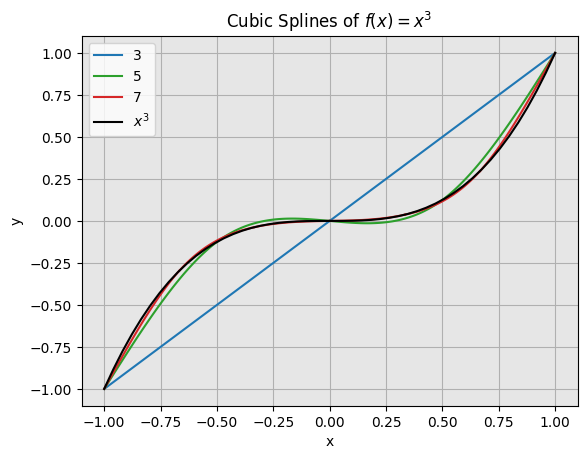
\includegraphics[width = 0.6\textwidth]{Plots/Exercise 26a.png}
    \caption{Natural Cubic splines for the function $f(x) = x^3$ for given $N$.}
    \label{fig:Exercise 26a}
\end{figure}

\newpage
\subsection{Exercise 26, part 3}
Compare $s_N$ with the function $f(x) = x^3$. For which $x \in [-1, 1]$ is $|s_N - f(x)|$ maximized? why?
\partbreak
\begin{solution}

    The plot for the error of each cubic spline is given below. I have highlighted the maximum points for each spline. It is clear that for each maximum, there is an equal maximum mirrored across the $x$-axis. Furthermore, it seems as though the minimum distance between a max and its closest node is mirrored. 
    
\end{solution}
\vspace{1in}
\begin{figure}[!ht]
    \centering
    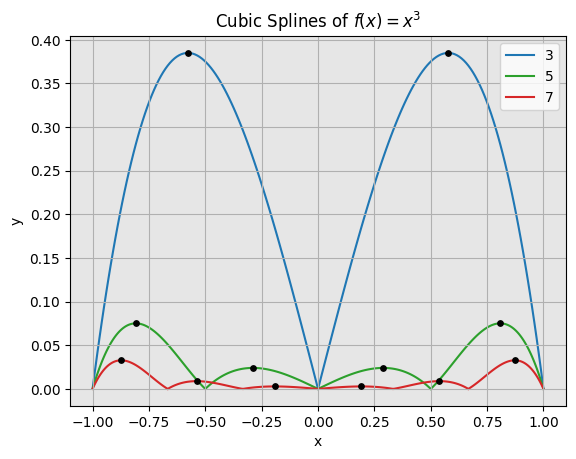
\includegraphics[width = 0.6\textwidth]{Plots/Exercise 26b.png}
    \caption{Error for each cubic spline for given orders. Maxes have been highlighted.}
    \label{fig:Exercise 26b}
\end{figure}

\newpage
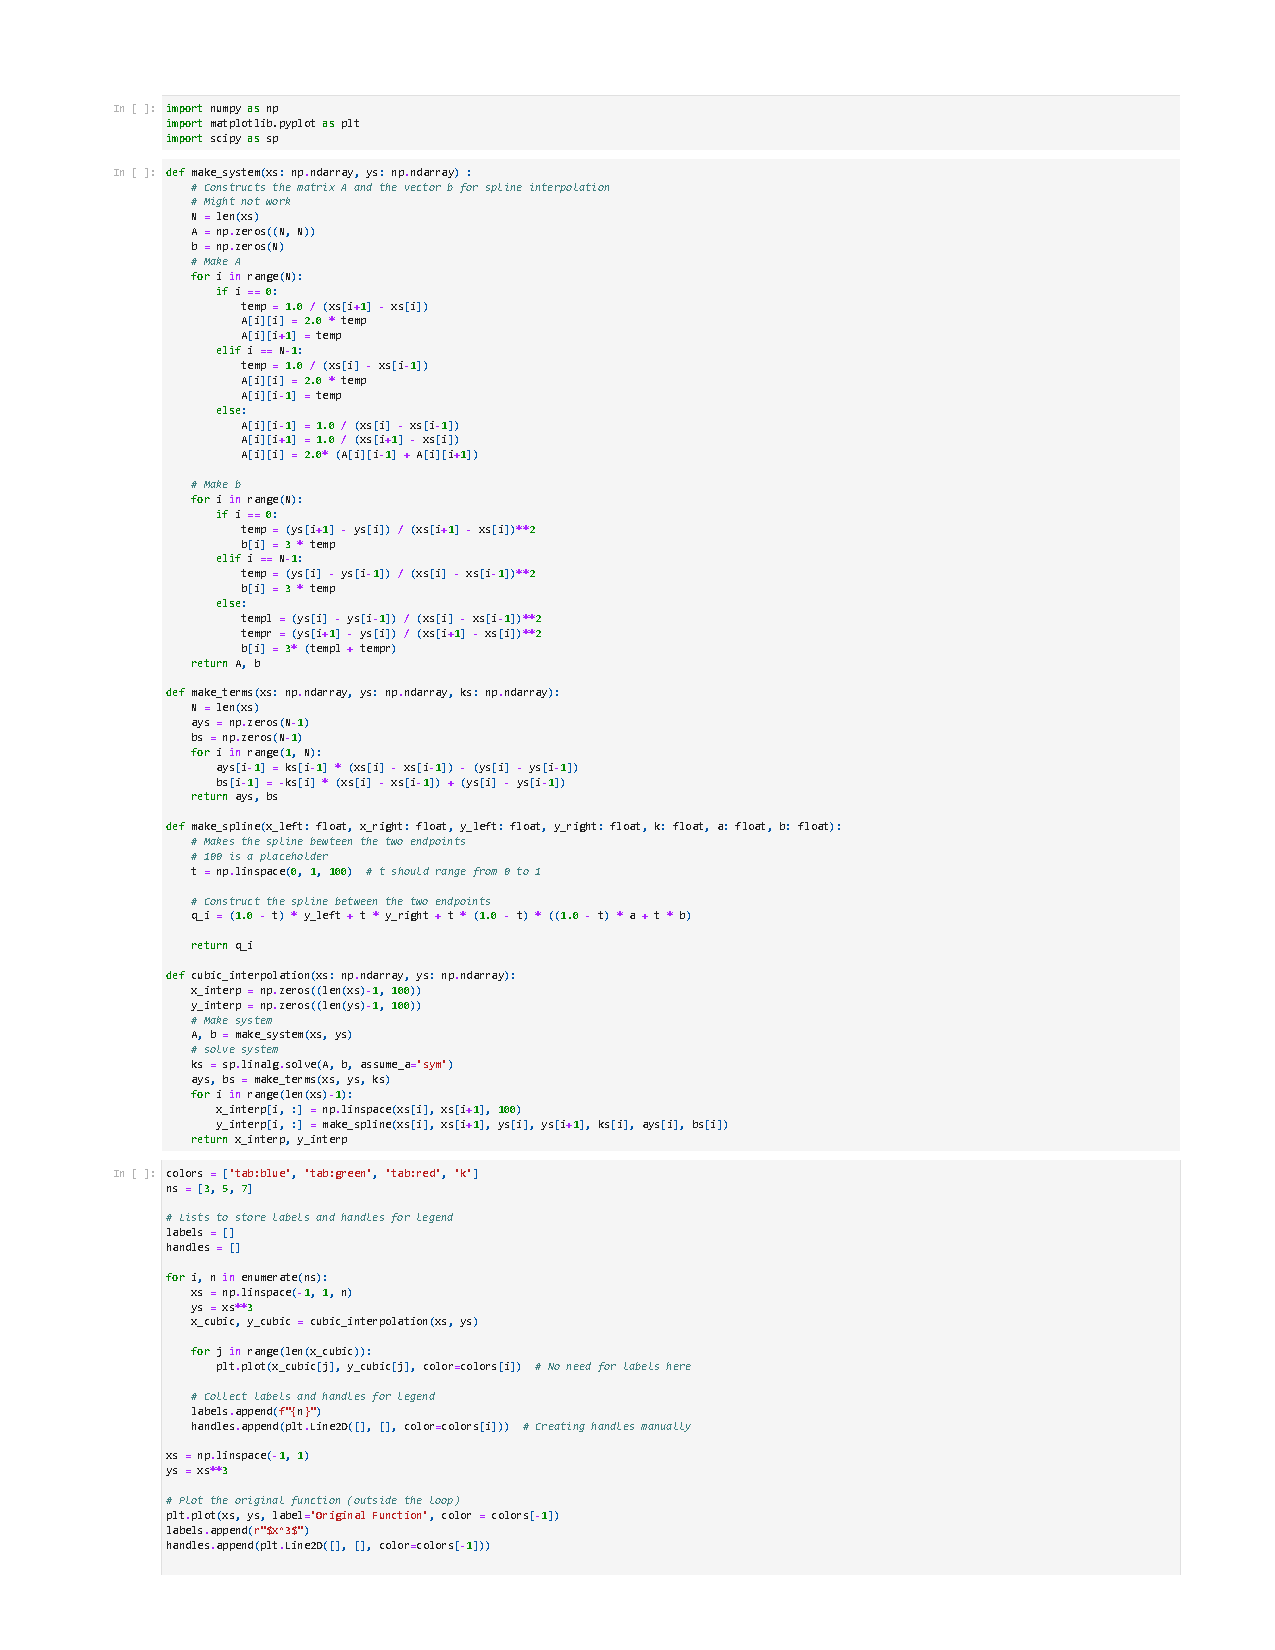
\includepdf[pages={1-}]{CodePDFs/Exercise26b.pdf}

\newpage
\subsection{Exercise 26, part 4}
(Open ended) Can you come up with an extension of 'natural' splines to higher-order? Do they satisfy an orthogonality condition like natural cubic splines? Can you write them in a 'radial basis function' type format? 
\end{document}